\chapter{希格斯機制：規範玻色子如何獲得質量}

現在我們把上一講介紹的兩個想法結合起來。具有破缺全域 \(U(1)\) 對稱性的複純量場，包含一個有質量的徑向振盪，以及一個無質量的角向振盪。局域不變的 \(U(1)\) 理論則包含一個無質量的規範場。當純量帶電，且其平衡幅值不為零時，這兩項陳述不能直接併在一起。角向模態與規範場結合：規範場因此有了質量，表面上的戈德斯通玻色子不再是獨立粒子，而徑向的希格斯模態仍然存在。

我們會以光子作為模型中的規範玻色子，但這不是我們要得出的物理結論。真空中的電磁 \(U(1)\) 並未破缺，因此真實的光子是無質量的。同一機制作用於電弱理論中的 \(W^\pm\) 和 \(Z\)；在該理論中，規範群和純量多重態都更為複雜。阿貝爾模型能清楚呈現這個機制，不會讓群論掩蓋它。

\begin{classroomqa}
\audiencequestion{先前的討論是否表示希格斯機制會賦予真實光子質量？\lecturetimestamp{00:00:23}}
\lecturerresponse{不會。我們問的是，\emph{如果}與光子相關的 \(U(1)\) 處於破缺相，會發生什麼事。那個假想的光子會變得有質量。真實的電磁真空並不處於該相；在粒子物理中的應用，指的是 \(W\) 和 \(Z\) 的質量。}
\end{classroomqa}

與電荷守恆相關的對稱性是相位旋轉
\begin{equation}
  \phi(x)\longmapsto e^{i\theta}\phi(x),
\end{equation}
這是一種稱為 \(U(1)\) 的內部旋轉。超導體提供了破缺相的實際類比。在超導體內部，電磁場有有限的穿透深度，在重要的方面表現得像有質量的場；在超導體外部，普通的無質量光子則重新出現。

\section{場的質量代表什麼}

\subsection{色散關係與零動量能隙}

在引入希格斯場之前，值得先明確說明我們所說的質量究竟是什麼意思。對波而言，
\begin{equation}
  E=\hbar\omega,
  \qquad
  p=\hbar k,
  \label{eq:l08-quantum-wave}
\end{equation}
因此，\((E,p)\) 圖和 \((\omega,k)\) 圖所含的資訊相同，只差了 \(\hbar\) 的因子。在真空中，無質量的相對論性激發滿足
\begin{equation}
  E=c|p|,
  \qquad
  \omega=c|k|.
  \label{eq:l08-massless-dispersion}
\end{equation}
\(k\) 的正負號代表相反的傳播方向。關鍵在於，\(\omega\) 會隨著 \(k\) 趨近於零。

有質量的相對論性粒子滿足
\begin{equation}
  E^2=c^2p^2+m^2c^4.
  \label{eq:l08-massive-dispersion}
\end{equation}
在單位制 \(c=\hbar=1\) 下，
\begin{equation}
  \omega^2=k^2+m^2.
\end{equation}
當 \(k=0\) 時，能量為 \(E=mc^2\)；以自然單位制表示，就是 \(m\)。因此，質量就是零動量模態具有的非零能隙。

\begin{figure}[htbp]
\centering
\begin{adjustbox}{max width=\linewidth}
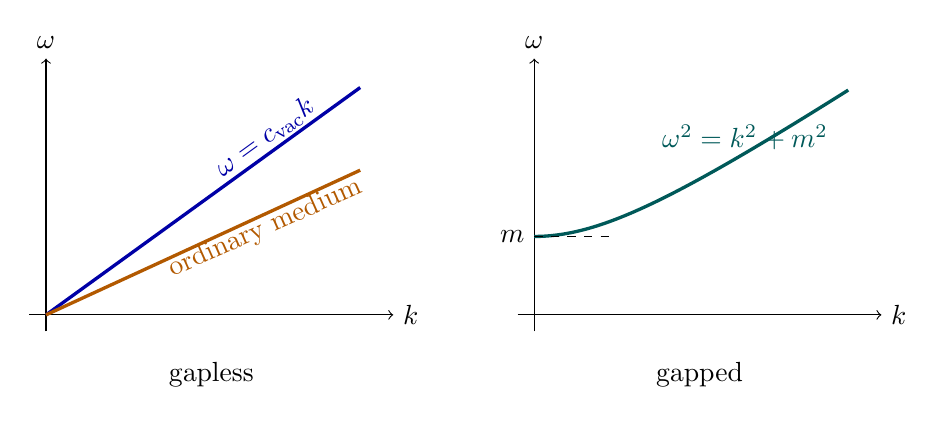
\begin{tikzpicture}[x=1.05cm,y=1.05cm]
  \begin{scope}
    \draw[->] (-0.2,0) -- (4.2,0) node[right] {\(k\)};
    \draw[->] (0,-0.2) -- (0,3.1) node[above] {\(\omega\)};
    \draw[very thick,blue!65!black] (0,0) -- (3.8,2.75);
    \draw[very thick,orange!70!black] (0,0) -- (3.8,1.75);
    \node[blue!65!black,rotate=36] at (2.65,2.15)
      {\(\omega=c_{\rm vac}k\)};
    \node[orange!70!black,rotate=24] at (2.65,1.05)
      {ordinary medium};
    \node[below] at (2,-0.45) {gapless};
  \end{scope}
  \begin{scope}[xshift=6.2cm]
    \draw[->] (-0.2,0) -- (4.2,0) node[right] {\(k\)};
    \draw[->] (0,-0.2) -- (0,3.1) node[above] {\(\omega\)};
    \draw[very thick,domain=0:3.8,samples=120,smooth,teal!70!black]
      plot (\x,{sqrt(0.9+0.45*\x*\x)});
    \draw[dashed] (0,0.95) -- (1.0,0.95);
    \node[left] at (0,0.95) {\(m\)};
    \node[teal!70!black] at (2.55,2.15)
      {\(\omega^2=k^2+m^2\)};
    \node[below] at (2,-0.45) {gapped};
  \end{scope}
\end{tikzpicture}
\end{adjustbox}
\caption{改變傳播速度會改變無能隙色散關係的斜率；賦予激發質量，則會在 \(k=0\) 處形成非零能隙。}
\label{fig:l08-dispersion}
\end{figure}

普通透明材料可以降低波的相速度，卻不會因此形成這種相對論性的質量能隙。在介面上，入射波的頻率固定，波數則會依照介質的色散關係調整。改變斜率與抬高截距並不相同。
\editorialnote{材料可能有多個電磁分支，而電漿或共振介質可能具有非零的電漿頻率能隙。本講比較的特定對象，是普通折射分支與超導響應。更一般地說，無能隙表示當 \(k\to0\) 時，\(\omega(k)\to0\)；在非相對論介質中，並非每種情況都必須嚴格線性。}

\begin{classroomqa}
\audiencequestion{光子只要穿過物質，例如稜鏡，就會獲得質量嗎？\lecturetimestamp{00:03:02}}
\lecturerresponse{不會。折射可以改變頻率與波數的關係，因而改變傳播速度，但該分支仍會在 \(\omega=0\) 處通過，且此時 \(k=0\)。超導相則會使電磁響應具有有限的穿透深度倒數，這是質量的類比。}
\end{classroomqa}

\begin{classroomqa}
\audiencequestion{固定頻率的光進入玻璃時，改變的是波數嗎？\lecturetimestamp{00:09:20}}
\lecturerresponse{是。靜止介面具有時間平移不變性，因此頻率維持不變。玻璃中的色散曲線斜率不同，所以相同的 \(\omega\) 對應不同的 \(k\)，波長也因此不同。}
\end{classroomqa}

斜率
\begin{equation}
  v_g=\frac{d\omega}{dk}
\end{equation}
是波包的群速度。如果斜率隨 \(k\) 改變，不同的傅立葉分量就會以不同速度移動，波包也會發生色散。這就是為什麼關係式 \(\omega(k)\) 稱為\emph{色散關係}。

\begin{classroomqa}
\audiencequestion{這條曲線叫什麼？它的斜率代表什麼？\lecturetimestamp{00:11:02}}
\lecturerresponse{這條曲線是色散關係，其導數
\(d\omega/dk\) 就是群速度。斜率固定時，各種波長的波以相同速度傳播；斜率變化時，波包便會展開。就目前的討論而言，關鍵差別在於曲線是否通過原點，或是具有能隙。}
\end{classroomqa}

\subsection{均勻振盪對應於靜止粒子}

\(k=0\) 模態的波長無限長：場在各處都偏移相同的量。讓均勻偏移開始振盪。如果場以非零頻率振盪，相應的量子便有非零靜止能量，也就是有質量。如果該方向沒有回復力，頻率就會是零，模態也就是無質量的。

這是經典的陳述，不要求空間上彼此分離的粒子處於量子疊加態。均勻的經典場組態，只是在整個空間中重複同一個場值。

\begin{classroomqa}
\audiencequestion{如果整個場一起偏移，這和量子糾纏是同一回事嗎？\lecturetimestamp{00:10:04}}
\lecturerresponse{不是。均勻的經典場是單一的經典組態。糾纏關聯的是不同的量子可能狀態，例如自旋向上--向下與自旋向下--向上的組態。在許多位置準備相同的場值，本身並不構成糾纏，也不代表存在瞬時的因果作用。}
\end{classroomqa}

對於正則歸一化的實場，
\begin{equation}
  \mathcal L
  =\frac12\partial_\mu\varphi\,\partial^\mu\varphi-V(\varphi),
\end{equation}
在平衡點 \(\varphi_0\) 附近展開：
\begin{equation}
  V(\varphi_0+\eta)
  =V(\varphi_0)
   +\frac12V''(\varphi_0)\eta^2+\cdots.
\end{equation}
線性項在極小值處消失，而場方程給出
\begin{equation}
  \omega^2=\bm{k}^2+m^2,
  \qquad
  m^2=V''(\varphi_0).
  \label{eq:l08-curvature-mass}
\end{equation}
因此，質量是勢能沿運動方向的曲率。平坦方向的曲率為零，因而產生無質量模態。

\section{破缺的複純量}

\subsection{徑向與角向運動}

將複純量以直角座標和極座標表示：
\begin{equation}
  \phi=\phi_R+i\phi_I=\rho e^{i\alpha},
  \qquad
  \phi^*=\phi_R-i\phi_I=\rho e^{-i\alpha}.
  \label{eq:l08-polar-field}
\end{equation}
複平面是一個\emph{內部}場空間。在每個物理時空點 \(x\)，這一對
\((\phi_R(x),\phi_I(x))\) 指定內部平面中的一個點。內部平面的兩個軸都不是實驗室中的空間方向。

\begin{figure}[htbp]
\centering
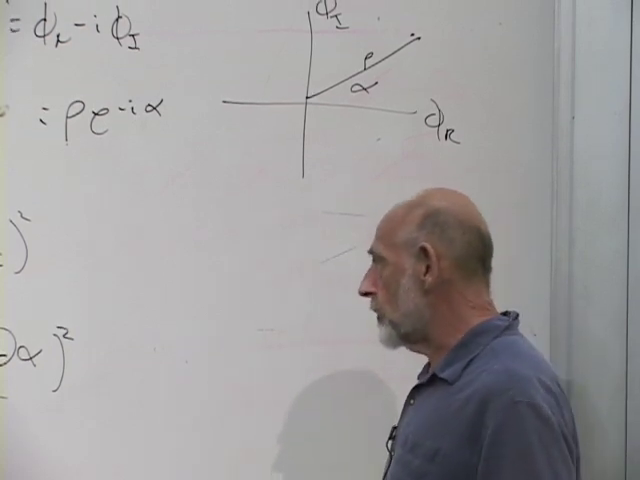
\includegraphics[width=0.72\textwidth]{lecture_08_figure_02.png}
\caption{複純量在內部 \((\phi_R,\phi_I)\) 平面上的表示。半徑為 \(\rho\)，\(\alpha\) 則是內部相位。}
\lectureframe{00:24:41}
\label{fig:l08-internal-plane}
\end{figure}

純量的動能項變為
\begin{align}
  \partial_\mu\phi^*\,\partial^\mu\phi
  &=
  \partial_\mu\phi_R\,\partial^\mu\phi_R
  +\partial_\mu\phi_I\,\partial^\mu\phi_I
  \notag\\
  &=
  \partial_\mu\rho\,\partial^\mu\rho
  +\rho^2\partial_\mu\alpha\,\partial^\mu\alpha.
  \label{eq:l08-polar-kinetic}
\end{align}
全域 \(U(1)\) 不變的勢能取決於 \(\phi^*\phi=\rho^2\)，而不取決於 \(\alpha\)。例如，
\begin{equation}
  V(\phi)
  =\lambda\left(\phi^*\phi-\frac{f^2}{2}\right)^2,
  \qquad \lambda>0.
  \label{eq:l08-mexican-hat}
\end{equation}
勢能的極小值構成一個圓。定律在共同的相位旋轉下保持不變，但選定一個平衡相位，就等於選定圓上的一個點。

\begin{figure}[htbp]
\centering
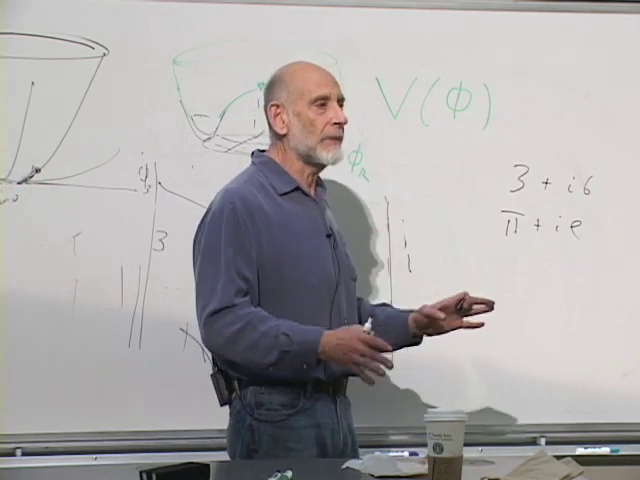
\includegraphics[width=0.78\textwidth]{lecture_08_figure_03.png}
\caption{黑板上的徑向勢能示意圖。勢能在內部場值旋轉下保持對稱，即使場本身不一定位於原點。}
\lectureframe{00:34:22}
\label{fig:l08-radial-potential-board}
\end{figure}

\begin{figure}[htbp]
\centering
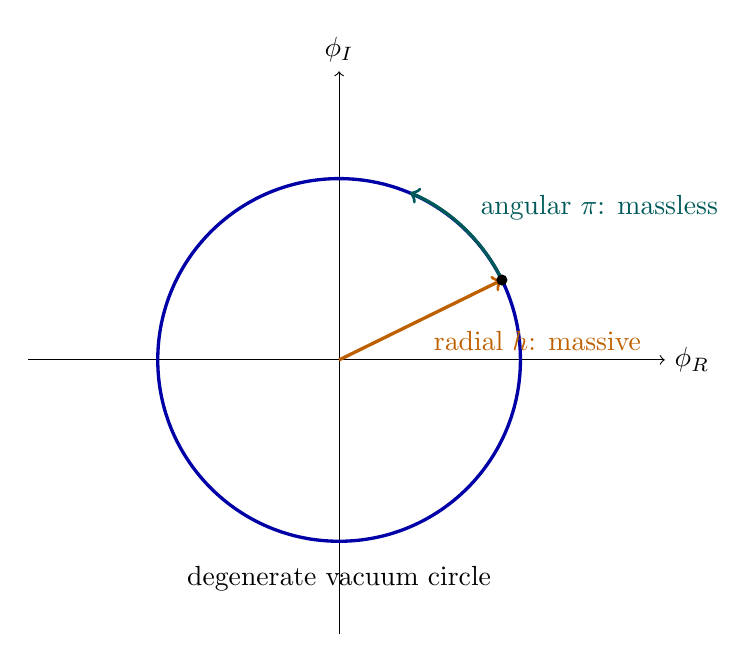
\begin{tikzpicture}[x=0.94cm,y=0.94cm]
  \draw[->] (-4.2,0) -- (4.4,0) node[right] {\(\phi_R\)};
  \draw[->] (0,-3.7) -- (0,3.9) node[above] {\(\phi_I\)};
  \draw[very thick,blue!65!black] (0,0) circle (2.45);
  \draw[->,very thick,orange!75!black] (0,0) -- (2.2,1.08);
  \draw[->,very thick,teal!70!black]
    (2.2,1.08) arc[start angle=26,end angle=67,radius=2.45];
  \node[orange!75!black,below right] at (1.15,0.52)
    {radial \(h\): massive};
  \node[teal!70!black,above right] at (1.78,1.76)
    {angular \(\pi\): massless};
  \fill (2.2,1.08) circle (2pt);
  \node[below] at (0,-2.65) {degenerate vacuum circle};
\end{tikzpicture}
\caption{全域對稱性破缺後的理論，在垂直於真空圓的方向上有曲率，沿著圓周的方向則沒有曲率。徑向希格斯模態有質量；角向戈德斯通模態無質量。}
\label{fig:l08-radial-angular}
\end{figure}

令
\begin{equation}
  \phi(x)=\frac{f+h(x)}{\sqrt2}
           e^{i\pi(x)/f}.
  \label{eq:l08-canonical-polar}
\end{equation}
在選定的真空附近，\(h\)表示徑向位移，\(\pi\)則以正則量綱表示切向位移。代入式~\eqref{eq:l08-polar-kinetic}，得到
\begin{equation}
  \partial_\mu\phi^*\,\partial^\mu\phi
  =
  \frac12(\partial_\mu h)^2
  +\frac12\left(1+\frac{h}{f}\right)^2
            (\partial_\mu\pi)^2.
  \label{eq:l08-global-expanded}
\end{equation}
式~\eqref{eq:l08-mexican-hat}的勢能給出
\begin{equation}
  m_h^2=2\lambda f^2,
  \qquad
  m_\pi^2=0.
  \label{eq:l08-global-masses}
\end{equation}
在遠低於 \(m_h\) 的能量下，徑向運動所需的能量很高，因此我們可以暫時固定 \(h=0\)。剩下的拉格朗日量只含有 \(\frac12(\partial\pi)^2\)，沒有 \(\pi^2\) 項。這就是戈德斯通玻色子。\editorialnote{口頭說明有兩處把名稱顛倒，並說是戈德斯通玻色子被吸收後，希格斯玻色子才有質量。黑板上的計算以及本講其餘內容表明，正確的結果是：徑向曲率已使希格斯模態具有質量，而規範玻色子吸收戈德斯通模態後變得有質量。}

\begin{classroomqa}
\audiencequestion{這是標準模型中唯一的自發對稱性破缺嗎？\lecturetimestamp{00:16:39}}
\lecturerresponse{與此處相關且已確立的對稱性破缺機制，是電弱希格斯相。其實際對稱性是 \(SU(2)_L\times U(1)_Y\)，而非單一的 \(U(1)\)；QCD 也有其他真空結構，例如手徵對稱性破缺。這個阿貝爾例子是刻意簡化的規範玻色子機制模型。}
\end{classroomqa}

\begin{classroomqa}
\audiencequestion{希格斯會賦予所有粒子質量嗎？它自己也包括在內嗎？\lecturetimestamp{00:17:11}}
\lecturerresponse{這個問題需要分兩方面回答。電弱對稱性禁止 \(W\)、\(Z\) 和標準模型費米子具有裸質量；它們的質量是在希格斯場取得非零平衡幅值後才出現。徑向希格斯模態的質量來自希格斯場自身勢能的曲率。其他假想粒子則可能具有對稱性所允許、與此機制無關的質量。}
\end{classroomqa}

本講將這類對稱性允許的質量，與可能非常重而難以觀測的粒子聯繫起來，並以暗物質作為可能的例子。這只是提出問題的動機，並非對質量的預測。
\editorialnote{暗物質的質量尺度仍然未知。本講提到粒子質量約為質子質量一千倍，這是過去的推測，並非經實驗確立的暗物質性質。}

\begin{classroomqa}
\audiencequestion{\(\rho\)是物理半徑，還是場值？究竟什麼具有徑向對稱性？\lecturetimestamp{00:33:08}}
\lecturerresponse{在每個時空點，場值都是輔助複平面中的一個點，而 \(\rho=|\phi|\) 是該點到原點的距離。\emph{勢能}在這個內部平面上具有徑向對稱性：所有 \(\rho\) 相同的點，其勢能也相同。這個半徑不是普通空間中的距離。}
\end{classroomqa}

\begin{classroomqa}
\audiencequestion{如果徑向踢動足夠劇烈，能否讓場越過中央極大值，到達勢能的另一側？
\lecturetimestamp{00:36:00}}
\lecturerresponse{原則上，局部組態若有足夠能量，就能越過位能障壁。要讓均勻的宏觀場越過障壁，需要極大的能量；一般的劇烈擾動也會把能量分散到許多場模態中，不會相干地抵達另一側的點。低能近似會固定 \(\rho\)，正是因為在該近似適用的能量範圍內，無法進行這種徑向偏移。}
\end{classroomqa}

\section{為什麼複平面不是時空}

物理座標與內部座標的區別，值得像本講那樣特別停下來說明。純量場之所以稱為純量，是因為它在物理座標軸旋轉時保持不變。兩個實純量場 \(\phi_R(x)\) 和 \(\phi_I(x)\) 在這種旋轉下仍是兩個純量。我們可以把它們合寫成一個複數，但這種記號安排不會使它們變成空間向量的分量。

全域 \(U(1)\) 變換會旋轉場的 \emph{值}：
\begin{equation}
\begin{aligned}
  \phi(x)&\longmapsto e^{i\theta}\phi(x),
  \\
  \rho(x)&\longmapsto\rho(x),
  \\
  \alpha(x)&\longmapsto\alpha(x)+\theta.
\end{aligned}
  \label{eq:l08-global-shift}
\end{equation}
同一個常數 \(\theta\) 用於每個時空點，因此 \(\partial_\mu\alpha\) 保持不變。勢能和一般的動能項都具有這項對稱性。一旦允許 \(\theta\) 隨 \(x\) 改變，導數就會察覺這項變化，論證也就不同了。

\section{將相位旋轉改為局域變換}

\subsection{一般導數不再適用}

令
\begin{equation}
  \phi'(x)=e^{i\theta(x)}\phi(x).
  \label{eq:l08-local-phase}
\end{equation}
則
\begin{equation}
  \partial_\mu\phi'
  =e^{i\theta}
    \left(\partial_\mu\phi+i\,\partial_\mu\theta\,\phi\right).
  \label{eq:l08-ordinary-derivative-fails}
\end{equation}
其中與 \(\partial_\mu\theta\) 成正比的額外項，使 \(\partial_\mu\phi\) 不會像 \(\phi\) 那樣變換。因此，\(\partial_\mu\phi^*\partial^\mu\phi\) 並非在任意局域相位旋轉下都保持不變。

\begin{figure}[htbp]
\centering
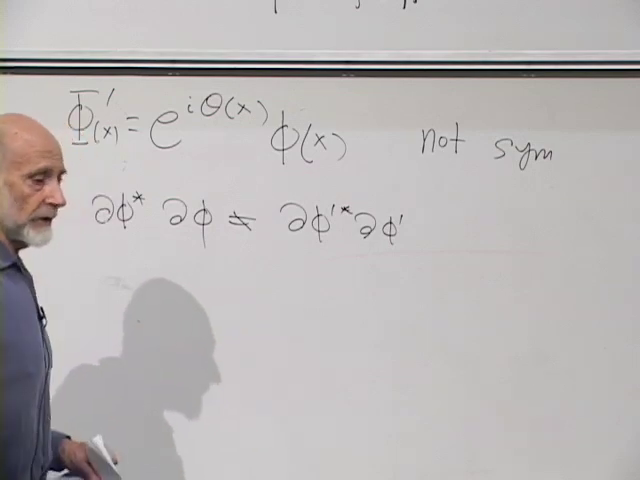
\includegraphics[width=0.78\textwidth]{lecture_08_figure_04.png}
\caption{黑板記下局域相位變換，以及一般導數項無法維持不變的情形。}
\lectureframe{00:46:49}
\label{fig:l08-local-not-symmetry}
\end{figure}

引入一個向量勢，並一致採用以下約定：
\begin{equation}
  D_\mu=\partial_\mu+i g A_\mu,
  \qquad
  A_\mu'=A_\mu-\frac1g\partial_\mu\theta.
  \label{eq:l08-covariant-convention}
\end{equation}
此時
\begin{align}
  D_\mu'\phi'
  &=
  \left(\partial_\mu+i g A_\mu'\right)
  e^{i\theta}\phi
  \notag\\
  &=
  e^{i\theta}
  \left[
    \partial_\mu\phi+i(\partial_\mu\theta)\phi
    +i g A_\mu\phi-i(\partial_\mu\theta)\phi
  \right]
  \notag\\
  &=e^{i\theta}D_\mu\phi.
  \label{eq:l08-covariant-transform}
\end{align}
不需要的項便會互相抵消。共軛導數為
\begin{equation}
  (D_\mu\phi)^*
  =(\partial_\mu-i g A_\mu)\phi^*,
\end{equation}
兩者的相位相反，因此在乘積中會抵消：
\begin{equation}
  (D_\mu\phi)^*D^\mu\phi.
\end{equation}

\begin{classroomqa}
\audiencequestion{上一講寫出的規範場變換，符號是否相反？\lecturetimestamp{00:48:04}}
\lecturerresponse{同時反轉 \(D_\mu\) 的符號和變換律中的符號，只是採用不同的約定。在 \(D_\mu=\partial_\mu+i gA_\mu\) 和 \(\phi'=e^{i\theta}\phi\) 的約定下，為保持一致，必須有 \(A_\mu'=A_\mu-g^{-1}\partial_\mu\theta\)。只要所有符號一起改變，另一種約定也同樣成立。}
\end{classroomqa}

\begin{classroomqa}
\audiencequestion{黑板上 \(\phi\) 的大寫或小寫寫法，是否代表不同的場？\lecturetimestamp{00:55:02}}
\lecturerresponse{這裡沒有要區分兩者。字母形狀不同只是手寫造成的，並不表示有額外的運算或第二個純量。真正有意義的區別是撇號、複共軛星號和時空指標。}
\end{classroomqa}

\begin{classroomqa}
\audiencequestion{動能項中的複共軛，和洛倫茲指標的升降是同一種運算嗎？
\lecturetimestamp{00:56:50}}
\lecturerresponse{不是。星號表示對內部的複數場取共軛。洛倫茲指標則以時空度規升降：\(D^\mu=g^{\mu\nu}D_\nu\)。要得到洛倫茲純量，必須作縮併 \((D_\mu\phi)^*D^\mu\phi\)。這兩種運算都會出現，但用途不同。}
\end{classroomqa}

\subsection{規範場也有自身的動力學}

場強
\begin{equation}
  F_{\mu\nu}=\partial_\mu A_\nu-\partial_\nu A_\mu
  \label{eq:l08-field-strength}
\end{equation}
具有規範不變性，因為 \(\theta\) 的兩個混合二階導數會互相抵消。它的時間--空間分量包含電場，空間--空間分量則包含磁場。因此，純量電動力學的拉格朗日量為
\begin{equation}
  \mathcal L
  =(D_\mu\phi)^*D^\mu\phi
  -V(\phi^*\phi)
  -\frac14F_{\mu\nu}F^{\mu\nu}.
  \label{eq:l08-abelian-higgs}
\end{equation}
這裡的帶電場是玻色場，不是作為費米子的電子場。帶電的氦原子核或庫珀對凝聚體，都是帶電玻色自由度可能出現的例子。

對稱性破缺之前，規範場項包含 \(A_\mu\) 的導數，卻沒有直接的質量項。或許可以試著加入
\begin{equation}
  \frac12m_A^2A_\mu A^\mu,
\end{equation}
但根據式 ~\eqref{eq:l08-covariant-convention}，
\begin{equation}
  A_\mu A^\mu
  \longmapsto
  \left(A_\mu-\frac1g\partial_\mu\theta\right)
  \left(A^\mu-\frac1g\partial^\mu\theta\right),
  \label{eq:l08-bare-mass-fails}
\end{equation}
這不等於 \(A_\mu A^\mu\)。局域對稱性禁止規範玻色子具有裸質量。

\begin{figure}[htbp]
\centering
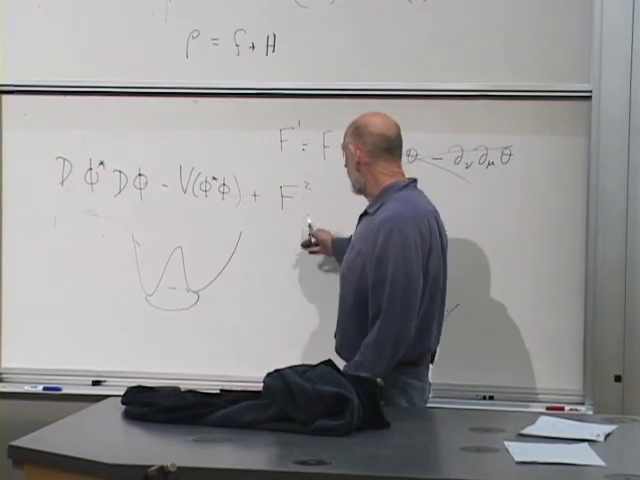
\includegraphics[width=0.76\textwidth]{lecture_08_figure_05.png}
\caption{經確認的黑板內容呈現了這項障礙：在規範變換下，\(A_\mu A^\mu\) 會變成一個包含 \(\partial_\mu\theta\) 的平方項，因此裸向量質量項並非不變量。}
\lectureframe{01:07:30}
\label{fig:l08-bare-mass-board}
\end{figure}

\section{希格斯機制}

\subsection{協變導數如何產生質量}

回到對稱性破缺的勢能，採用正則歸一化的參數表示
\begin{equation}
  \phi(x)=\frac{f+h(x)}{\sqrt2}
  e^{i\pi(x)/f}.
\end{equation}
其協變導數為
\begin{equation}
  D_\mu\phi
  =
  \frac{e^{i\pi/f}}{\sqrt2}
  \left[
    \partial_\mu h
    +i(f+h)
      \left(\frac{\partial_\mu\pi}{f}+gA_\mu\right)
  \right].
  \label{eq:l08-covariant-polar}
\end{equation}
因此，
\begin{equation}
\begin{aligned}
  (D_\mu\phi)^*D^\mu\phi
  ={}&
  \frac12(\partial_\mu h)^2
  \\
  &+\frac12(f+h)^2
    \left(\frac{\partial_\mu\pi}{f}+gA_\mu\right)
  \\
  &\hspace{4.2em}\times
    \left(\frac{\partial^\mu\pi}{f}+gA^\mu\right).
\end{aligned}
  \label{eq:l08-higgs-kinetic}
\end{equation}

關鍵項在作任何規範選擇之前就已出現：
\begin{equation}
  \frac12g^2f^2 A_\mu A^\mu.
  \label{eq:l08-vector-mass-term}
\end{equation}
與普羅卡形式 \(\frac12m_A^2A_\mu A^\mu\) 比較，可得
\begin{equation}
  \boxed{m_A=g f}.
  \label{eq:l08-vector-mass}
\end{equation}
同一次展開也會產生交互作用項 \(g^2fh A_\mu A^\mu\) 和 \(\frac12g^2h^2A_\mu A^\mu\)。因此，向量質量並非任意破壞規範對稱性的結果，而是從規範不變的純量動能項產生；此項是在平衡幅值 \(f\) 不為零的相中計算。

\begin{figure}[htbp]
\centering
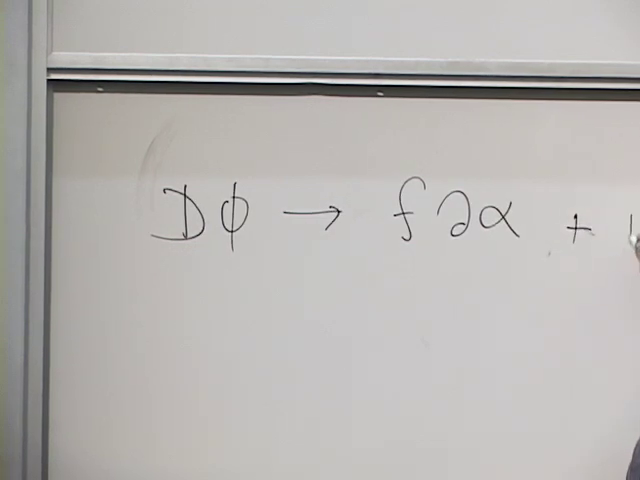
\includegraphics[width=0.78\textwidth]{lecture_08_figure_06.png}
\caption{黑板從 \((D\phi)^*(D\phi)\) 中分離出 \(f^2A^2\) 項。在式 ~\eqref{eq:l08-canonical-polar} 和 \eqref{eq:l08-covariant-convention} 所採用的歸一化下，結果為 \(m_A=gf\)；數值因子會依純量場和規範耦合常數的歸一化方式而異。}
\lectureframe{01:10:10}
\label{fig:l08-generated-mass-board}
\end{figure}

講座將 \(g\) 和數個 \(\sqrt2\) 因子吸收到黑板記號中，因此在標示質量時，短暫地交替使用 \(f\)、\(2f\) 和 \(\sqrt2f\)。除非先說明動能項和勢能的歸一化方式，否則這些因子並沒有不依賴約定的意義。穩健的結果是 \(m_A\propto gf\)；式 ~\eqref{eq:l08-vector-mass} 給出了此處採用的約定所對應的因子。

\subsection{吸收相位}

在規範變換下，相位變數的變化為
\begin{equation}
  \pi'(x)=\pi(x)+f\,\theta(x).
\end{equation}
選擇
\begin{equation}
  \theta(x)=-\frac{\pi(x)}{f}.
  \label{eq:l08-unitary-gauge-choice}
\end{equation}
便有 \(\pi'=0\)。這就是么正規範；在此規範下，\begin{equation}
  \phi'(x)=\frac{f+h(x)}{\sqrt2}
\end{equation} 為實數，而式 ~\eqref{eq:l08-higgs-kinetic} 化為
\begin{equation}
  (D_\mu\phi')^*D^\mu\phi'
  =
  \frac12(\partial_\mu h)^2
  +\frac12g^2(f+h)^2A_\mu'A^{\prime\mu}.
  \label{eq:l08-unitary-gauge-lagrangian}
\end{equation}
角向戈德斯通場不再是獨立變數，但向量質量仍然存在。

講座先在低能極限 \(\rho=f\) 下展示這一點，此時
\begin{align}
  \phi&=f e^{i\alpha},
  \notag\\
  D_\mu\phi
  &=if e^{i\alpha}
    \left(\partial_\mu\alpha+gA_\mu\right),
  \notag\\
  (D_\mu\phi)^*
  &=-if e^{-i\alpha}
    \left(\partial_\mu\alpha+gA_\mu\right).
  \label{eq:l08-frozen-radius}
\end{align}
兩者相乘得到
\begin{equation}
  f^2
  \left(\partial_\mu\alpha+gA_\mu\right)
  \left(\partial^\mu\alpha+gA^\mu\right).
\end{equation}
選擇 \(\theta=-\alpha\) 後，便剩下 \(g^2f^2A_\mu'A^{\prime\mu}\)。

\begin{figure}[htbp]
\centering
\includegraphics[width=0.82\textwidth]{lecture_08_figure_07.png}
\caption{固定半徑下的完整板書狀態：協變導數同時包含相位導數與向量位勢。接著，講座中選取\(\theta=-\alpha\)以消去相位，留下向量質量項。}
\lectureframe{01:16:20}
\label{fig:l08-frozen-radius-board}
\end{figure}

\begin{classroomqa}
\audiencequestion{能否改用一組變數重寫整個拉格朗日量，讓角向模態如何消失一目了然？
\lecturetimestamp{01:13:49}}
\lecturerresponse{可以。在極座標變數中，相位只會透過規範不變的組合 \(\partial_\mu\alpha+gA_\mu\) 出現。作規範變換並取 \(\theta=-\alpha\)，就能在此規範定義良好的所有位置將相位設為零。如此一來，純量動能項便成為向量質量項，而規範不變的場強項維持不變。}
\end{classroomqa}

\begin{classroomqa}
\audiencequestion{\(\alpha\)中的振盪，和規範振盪無法區分嗎？\lecturetimestamp{01:18:02}}
\lecturerresponse{在規範化理論中，若 \(\alpha\) 的純粹變化由 \(A_\mu\) 的相應變化抵銷，那只是對規範的重新描述，不代表另一個物理波。規範不變的量是 \(\partial_\mu\alpha+gA_\mu\)。原先由全域戈德斯通場描述的物理模態，則成為有質量向量的縱向偏振。}
\end{classroomqa}

常有人說局域規範對稱性會自發破缺。就實際操作而言，這種說法很有用：選定規範後，純量場具有非零真空值，粒子譜中也會出現有質量的向量。不過嚴格來說，規範變換關聯的是冗餘描述，而非不同的物理態。
\editorialnote{局域規範冗餘並不像全域對稱性那樣，以規範不變的意義破缺。更精確地說，該理論處於希格斯相。固定規範後的微擾論，則以非零的純量期望值及由此產生的有質量向量粒子譜來描述這個相。}

\section{戈德斯通自由度去了哪裡}

改變變數不會讓任何物理自由度憑空消失。來比較進入希格斯相前後的自由度數目。

之前：
\begin{equation}
  \underbrace{2}_{\text{massless vector}}
  +
  \underbrace{2}_{\text{complex scalar}}
  =4.
\end{equation}
無質量向量有兩個橫向偏振；複純量則有兩個實分量，分別是徑向和角向分量。

之後：
\begin{equation}
  \underbrace{3}_{\text{massive vector}}
  +
  \underbrace{1}_{\text{radial Higgs}}
  =4.
  \label{eq:l08-degree-count}
\end{equation}
有質量的向量可以在其靜止系中描述。靜止系裡沒有任何空間方向特別突出，因此它必須有三種偏振態。向量運動時，其中兩種是橫向偏振，一種是縱向偏振。戈德斯通模態便成為這個縱向偏振。

\begin{figure}[htbp]
\centering
\begin{adjustbox}{max width=\linewidth}
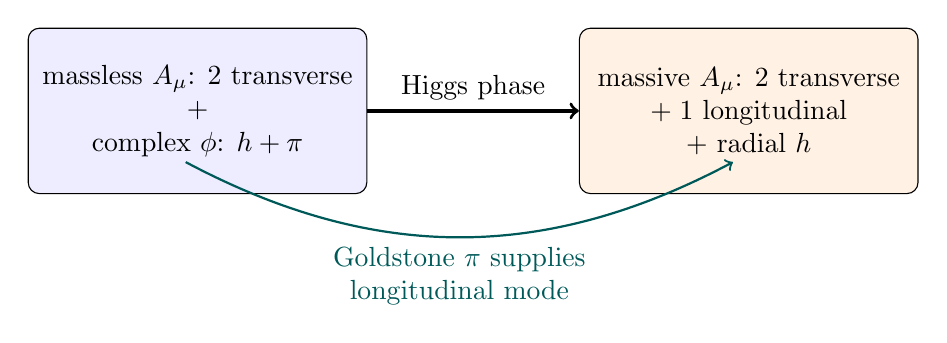
\begin{tikzpicture}[x=1cm,y=1cm]
  \node[draw,rounded corners,fill=blue!7,minimum width=4.3cm,
        minimum height=2.1cm,align=center] (before) at (0,0)
    {massless \(A_\mu\): \(2\) transverse\\
     \(+\)\\
     complex \(\phi\): \(h+\pi\)};
  \node[draw,rounded corners,fill=orange!10,minimum width=4.3cm,
        minimum height=2.1cm,align=center] (after) at (7,0)
    {massive \(A_\mu\): \(2\) transverse\\
     \(+\;1\) longitudinal\\
     \(+\) radial \(h\)};
  \draw[->,very thick] (before) -- node[above]{Higgs phase} (after);
  \draw[->,teal!70!black,thick]
    (-0.15,-0.65) to[bend right=28]
    node[below,align=center]{Goldstone \(\pi\) supplies\\longitudinal mode}
    (6.8,-0.65);
\end{tikzpicture}
\end{adjustbox}
\caption{希格斯機制重組了物理自由度，並未消滅它們。}
\label{fig:l08-degree-rearrangement}
\end{figure}

\begin{classroomqa}
\audiencequestion{角向自由度如何在不違反自由度計數的情況下消失？\lecturetimestamp{01:19:13}}
\lecturerresponse{它在物理上並沒有消失。無質量向量不能靜止，因此只有兩種螺旋度；有質量向量則有三種偏振，包括一種縱向偏振。戈德斯通模態成為第三種偏振，因此總自由度數目維持不變。}
\end{classroomqa}

講座提供了一個實用的運動學檢驗。設想一個有質量的向量粒子：先讓它減速至靜止，再沿新的方向加速。原本相對於舊運動方向為橫向的偏振，相對於新的運動方向可能變成縱向。同樣地，如果一個圓偏振的有質量粒子經過靜止，再沿相反方向運動，它的螺旋度標記就會反轉。嚴格無質量的粒子無法經歷這項實驗，因為任何慣性參考系都不能讓它靜止。因此，無質量粒子的兩種螺旋度構成一致的物理譜。

\section{超導體的類比}

在傳統超導體中，電子會形成庫珀對。每個庫珀對都是攜帶電荷 \(2e\) 的玻色子，而凝聚態則以帶電的複數序參量描述。當序參量的幅值不為零時，其相位與電磁向量勢結合，便產生安德森--希格斯機制。靜磁場會在倫敦穿透深度範圍內衰減，而不會自由延伸至超導體內部。就這個明確且依介質而定的意義而言，光子表現得彷彿獲得了質量。

這個例子也釐清了開頭提到的區別。電磁場並未永久轉變成另一種基本粒子。有質量的傳播定律適用於材料內部的集體態；在材料外部，真空中的光子仍是無質量的。

\section{目前得到的結論}

現在可以在不失去論證脈絡的前提下，將內容簡要整理如下：
\begin{enumerate}
  \item 全域連續對稱性破缺後，角向有一個平坦方向，因此會有無質量的戈德斯通模態。
  \item 局域相位不變性要求引入規範勢，並以 \(D_\mu\) 取代 \(\partial_\mu\)。
  \item 裸的 \(A_\mu A^\mu\) 質量違反局域變換律。
  \item 帶電純量的平衡幅值 \(f\) 不為零時，規範不變項 \(|D_\mu\phi|^2\) 會包含 \(\frac12g^2f^2A_\mu A^\mu\)。
  \item 選擇規範即可消去相位；相位所對應的物理自由度，會成為有質量向量的縱向偏振。
  \item 徑向希格斯激發仍然存在，其質量由純量勢能的曲率決定。
\end{enumerate}

接下來要說明費米子如何獲得質量。電子和夸克不能直接採用向量機制；它們透過湯川交互作用與希格斯場耦合。純量場穩定在 \(f\) 後，這些交互作用便成為費米子質量項。

「若沒有電弱對稱性破缺，我們熟悉的粒子都沒有質量」這個概括性的說法，還需要再加上一項限定。基本夸克和帶電輕子的質量，以及 \(W\) 和 \(Z\) 的質量，確實會隨希格斯期望值消失。然而，質子和中子的大部分質量來自 QCD 禁閉和強場能量的動力學效應，而非夸克的希格斯質量。這項區別不會改變此處推導的希格斯機制，只是讓我們更精確地界定它的適用範圍。
